\documentclass[11pt]{article}
\usepackage[margin=1in]{geometry}
\usepackage{graphicx}
\usepackage{booktabs}
\usepackage{hyperref}
\usepackage{float}
\usepackage{setspace}
\usepackage{caption}
\usepackage{amsmath}
\usepackage[numbers]{natbib}
\graphicspath{ {./image/} }

\title{QBS 103 Final Project Report}
\author{Ruiqi Li}
\date{\today}

\begin{document}
\maketitle

\section{Introduction}
The dataset used in this project comes from Overmyer \textit{et al.}, 2020, which profiled leukocyte gene expression in COVID-19 patients \citep{overmyer_large-scale_2021}. \\
For my main visualizations, I focused on the \textbf{A1BG} gene. A1BG (alpha-1-B glycoprotein) is expressed in human plasma, and I investigated its relationship with several clinical covariates, including age (continuous), sex (categorical), and ICU status (categorical). Additional covariates such as ferritin and CRP levels were also used for descriptive statistics and multivariate visualization. 

\section{Methods}
Data preprocessing and analysis were performed in R. Packages used included \texttt{ggplot2}, \texttt{dplyr}, \texttt{tidyr}, \texttt{pheatmap}, and \texttt{hexbin} \citep{ggplot22016,dplyr2023,R-tidyr,pheatmap2019,hexbin2022}. 
Counts were log$_2$-transformed with a pseudocount of 1 before visualization. \\
For the heatmap, I selected the top-variance genes (n=20), standardized them by row z-scores, and clustered rows and columns using Euclidean distance with complete linkage. \\
For two-dimensional visualization, I used hexagonal binning plots (\texttt{geom\_hex}) to summarize the relationship between age and gene expression values. This approach reduces overplotting by grouping nearby points into hexagonal bins and coloring them by the number of observations.



\section{Results}
\subsection{Table of summary statistics}
Table~\ref{tab:summary} summarizes baseline characteristics of the 126 participants stratified by ICU status at enrollment. \\
Categorical variables are reported as $n$ (\%), computed within each stratum: sex (female/male) and receipt of mechanical ventilation (Yes/No). \\
Continuous variables are summarized as mean (SD) for approximately symmetric distributions (age, CRP) and as median [IQR] for right-skewed measures (ferritin). \\
Sex labels were standardized to \textit{female}/\textit{male} after trimming whitespace; ICU status was harmonized from the original \textit{yes}/\textit{no} field; and mechanical ventilation indicates any documented ventilation during the index admission. \\
Overall, the ICU group was older on average than the Non-ICU group (63.5 vs.\ 58.7 years) and exhibited higher inflammatory markers: ferritin median 685 [325--1212] vs.\ 401 [131--870] ng/mL, and CRP mean 150 vs.\ 109 mg/L. Mechanical ventilation was markedly more frequent among ICU patients (69.7\% vs.\ 8.3\%). Sex distributions were broadly similar between strata (female: 36.9\% in ICU vs.\ 45.0\% in Non-ICU). 

\label{tab:summary}
\begin{table}[ht]
\centering
\caption{Summary statistics stratified by ICU status}
\begin{tabular}{lcc}
\hline
 & ICU (n = 66) & Non-ICU (n = 60) \\
\hline
\textbf{Categorical variables} & & \\
Sex, female & 24 (36.9\%) & 27 (45.0\%) \\
Sex, male   & 41 (63.1\%) & 33 (55.0\%) \\
Mechanical ventilation, Yes & 46 (69.7\%) & 5 (8.3\%) \\
Mechanical ventilation, No  & 20 (30.3\%) & 55 (91.7\%) \\
\hline
\textbf{Continuous variables} & & \\
Age, mean (SD) & 63.5 (14.0) & 58.7 (17.8) \\
Ferritin, median [IQR] & 685 [325--1212] & 401 [131--870] \\
CRP, mean (SD) & 150 (106) & 109 (94.4) \\
\hline
\end{tabular}
\end{table}

\subsection{Histogram of gene}
The histogram of A1BG expression (Figure~\ref{fig:hist}) shows a strongly right-skewed distribution with most observations concentrated at low values and a long, sparse upper tail. A small number of high-expression outliers are present, which widen the range but do not alter the overall pattern that the majority of samples exhibit modest expression. This shape suggests over-dispersion and potential zero/near-zero inflation that are typical for gene-level measurements; it also motivates the use of robust summaries (e.g., medians/IQRs) and transformations in downstream analyses.

\begin{figure}[H]
\centering
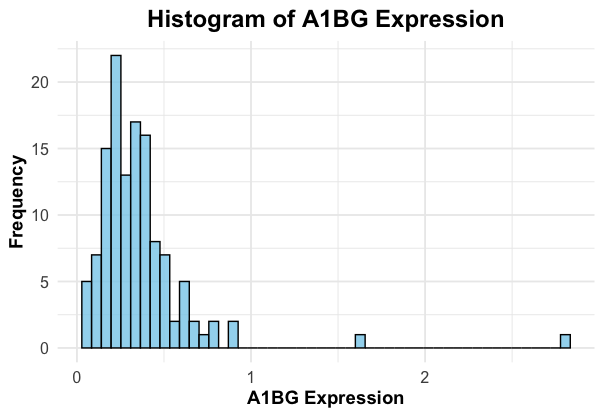
\includegraphics[width=0.7\textwidth]{fig1_hist.png}
\caption{Histogram of A1BG expression across all participants.}
\label{fig:hist}
\end{figure}

\newpage
\subsection{Scatter plot of gene + continuous covariate}
The A1BG–age scatterplot with a LOESS smoother (Figure~\ref{fig:scatter}) indicates no strong monotonic association between expression and age. The fitted curve is shallow and largely contained within the 95 percent confidence band, consistent with a weak or null relationship. Variability appears fairly constant across the age range, with a few isolated higher-expression points that do not align with a simple linear trend. Overall, these data do not provide evidence that A1BG expression changes meaningfully with age in this cohort.

\begin{figure}[H]
\centering
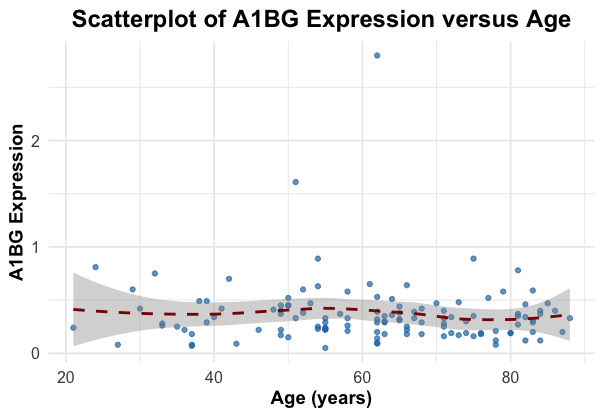
\includegraphics[width=0.75\textwidth]{fig2_scatter.png}
\caption{Scatter plot of A1BG expression vs.\ age with LOESS smoother; points colored by ICU status and shaped by sex.}
\label{fig:scatter}
\end{figure}

\subsection{Boxplot of gene stratified by two categorical covariates}
The boxplots stratified by sex and ICU status (Figure~\ref{fig:box}) show broadly similar A1BG expression between females and males, with overlapping interquartile ranges and comparable medians. When further grouped by ICU status (“yes” vs “no”), median differences remain small; non-ICU participants tend to have slightly higher central tendency, but the spread overlaps substantially across groups. The “unknown” sex category has very limited data (essentially a single value), so it should not be over-interpreted. Taken together, these comparisons suggest that large sex-specific differences are unlikely, and any ICU-related shifts in A1BG expression—if present—are modest.

\begin{figure}[H]
\centering
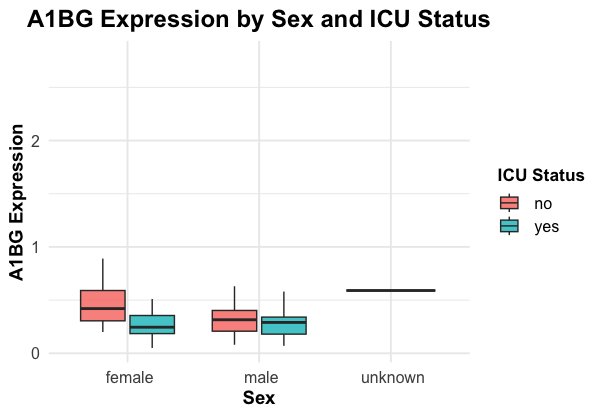
\includegraphics[width=0.62\textwidth]{fig3_box.png}
\caption{Boxplot of A1BG expression by sex and ICU status.}
\label{fig:box}
\end{figure}

\subsection{Heatmap}
The heatmap of the top variance genes (Figure~\ref{fig:heatmap}) summarizes multigene patterns after row z-scoring and hierarchical clustering. Column annotations reveal partial organization of samples by ICU status, with several gene blocks exhibiting coordinated up- or down-regulation among ICU subjects relative to non-ICU. Sex annotation shows no dominant block-level pattern, consistent with the boxplot findings. Because the visualization uses a subset of samples/genes and row scaling emphasizes relative (not absolute) differences, the heatmap highlights structure that is consistent with global disease-severity effects rather than single-gene changes.
\begin{figure}[H]
\centering
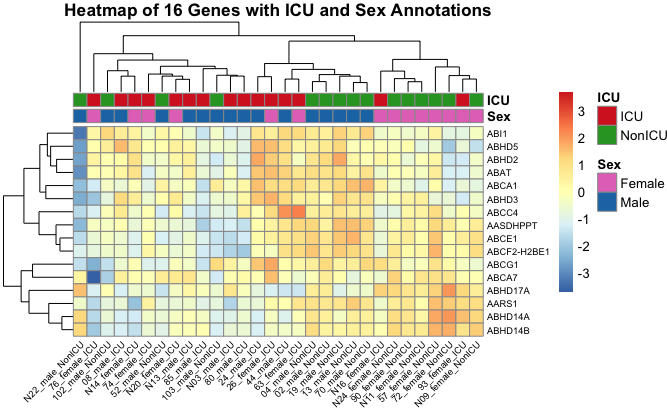
\includegraphics[width=0.75\textwidth]{fig4_heatmap.png}
\caption{Heatmap of the top 16 variance genes. Rows and columns are clustered with Euclidean distance and complete linkage. Annotation bars indicate sex and ICU status.}
\label{fig:heatmap}
\end{figure}

\subsection{New plot type (Hexbin)}

To provide a new view of the relationship between age and gene expression beyond the standard scatterplot, I used a \textbf{hexbin plot} implemented in \texttt{ggplot2::geom\_hex}. A hexbin plot partitions the 2D plane into small hexagonal cells and colours each cell by the number of observations it contains. This effectively solves overplotting when many points overlap and reveals the underlying \emph{density structure} of the data.

\paragraph{What is shown.}
Each panel displays patients from one ICU stratum (ICU vs.\ NonICU). The \textbf{x-axis} is age (years) and the \textbf{y-axis} is A1BG expression. The \textbf{colour scale} (legend ``Count'') indicates how many patients fall into each hexagonal bin; darker/brighter cells correspond to higher local density.

\paragraph{How it was produced.}
From the merged analysis dataset, I filtered records with finite age and A1BG values, harmonised ICU labels, and then drew:
\begin{itemize}
  \item \texttt{geom\_hex(bins = 28)} to create hexagonal bins (28 bins per axis; larger values give finer resolution).
  \item \texttt{facet\_wrap(\textasciitilde{} ICU)} to show ICU and NonICU side by side for direct comparison.
  \item \texttt{scale\_fill\_viridis\_c()} to apply a perceptually uniform colour scale for counts.
\end{itemize}

\paragraph{What it adds.}
Unlike a scatterplot that can obscure dense regions through overplotting, the hexbin view highlights \emph{where} observations concentrate. In this dataset, most patients cluster around ages $\sim$55--80 with A1BG expression in the $\sim$0.2--0.6 range across both strata, while a few sparse high-expression cells appear only in the NonICU panel, indicating rare outliers. The side-by-side panels make it easy to spot any shift in the bulk density between ICU and NonICU groups.

\begin{figure}[H]
\centering
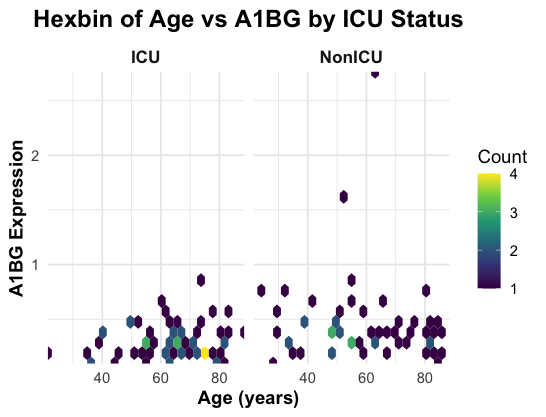
\includegraphics[width=0.7\textwidth]{fig5_hex.png}
\caption{Hexbin of Age vs A1BG Expression, stratified by ICU status.}
\label{fig:hex}
\end{figure}


\section{Discussion}
Overall, A1BG expression did not show strong associations with age or sex. 
However, patterns across multiple high-variance genes suggest global transcriptional changes in ICU patients (Figures~\ref{fig:heatmap}, \ref{fig:pca}). 
The PCA and heatmap provide complementary perspectives: the PCA summarizes global variance across samples, while the heatmap highlights gene-level differences.

\section{References}
\bibliographystyle{acm}
\bibliography{refs}
\end{document}
